\section{MetaMask}
	\subsection{What is MetaMask}
	MetaMask is a browser extensions that manages your Ethereum wallet and 
	allows you to send and receive Ethers (Cubits or CCs in \textit{Soldino}). 
	This plug-in is necessary to perform all the basic int this platform
	such as login and transactions. 
	\subsection{Installation}
	After entering \textit{Soldino}'s homepage check if you have MetaMask, 
	installed. You can check this by looking for its icon on the top right of 
	your browser
	\begin{figure}[H]
		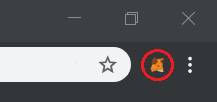
\includegraphics[width=7cm]{res/images/metamask_icon.png}
		\centering
		\caption{MetaMask's icon}
	\end{figure}
	\noindent If you have it proceed with the configuration of your account.
	Otherwise watch the video introduction, click the link under the video and 
	follow the instructions to download it. 
	\begin{figure}[H]
		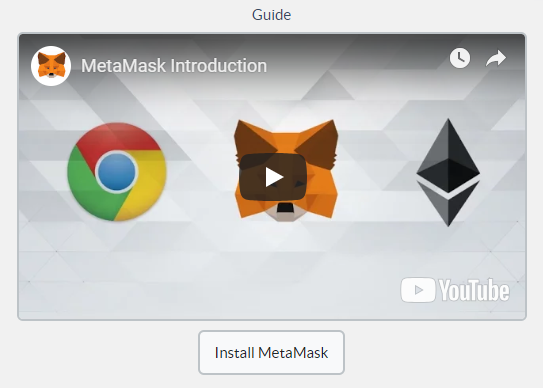
\includegraphics[width=7cm]{res/images/metamask_download.png}
		\centering
		\caption{Introduction to MetaMask}
	\end{figure}
	\noindent After the installation process is 
	complete you will see MetaMask's icon on the top right of your browser. A 
	new window will then open where you will have to configure your account.\\
	The download page can also be found at \url{https://metamask.io/}.
	
	\subsection{Configuration}
	Click on MetaMask's icon on the top right of your browser, and set up your 
	personal Ethereum wallet by following the instructions. You can either 
	create a new account or import an existing one from the 12 words seed phrase.
	\begin{figure}[H]
		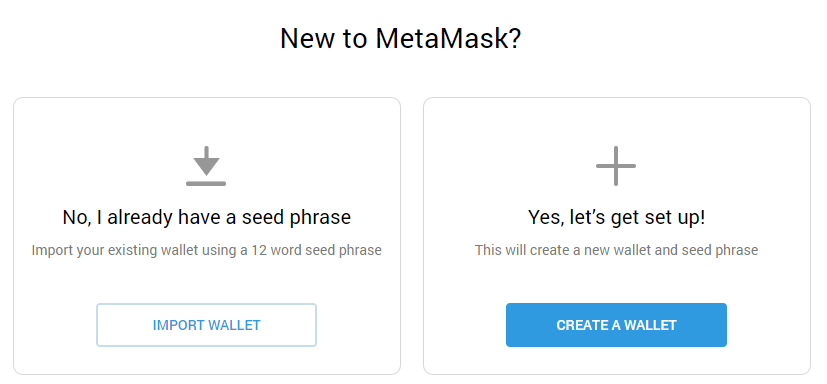
\includegraphics[width=10cm]{res/images/metamask_select.png}
		\centering
		\caption{MetaMask setup}
	\end{figure}
	\noindent After setting up your account you will be able to join and use 
	\textit{Soldino}.
	\newline \\
	Note that MetaMask has to be installed in your browser as long a you want 
	to use the platform: removing it from your browser will render you unable 
	to use \textit{Soldino}.
	\subsection{Transactions}
	Every time you make a transaction MetaMask will open a pop up window that 
	shows you its total cost.
	From this window you will be able to accept it or decline it.\\
	\begin{figure}[H]
		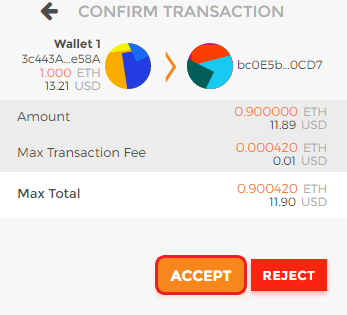
\includegraphics[width=10cm]{res/images/metamask_transaction.png}
		\centering
		\caption{Example of a MetaMask transaction}
	\end{figure}
	\noindent 
	Every change made on the Ethereum Network has a cost. This is called gas 
	and is measured in GWEI, a billionth of a Ether. When you make a 
	transaction you can choose whether it should have a high or low priority, 
	higher priority will consume more gas than a lower one but will be mined 
	quicker. We do not recommend changing the priority for transaction made 
	in \textit{Soldino} as it does not matter much.\\
	Note that all prices shown in the platform are in Cubits (CC), 
	\textit{Soldino}'s own special token. Also note that 1 Cubit = 1 Euro.
	%PLACEHOLDER mettere foto con tabella dei costi in gas